\chapter{Расчет биологической защиты}
\section{Постановка задачи}

\section{Постановка задачи}

\begin{figure}[!h]
	\center
	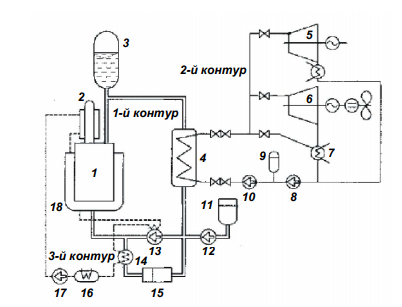
\includegraphics{media/image1.png}
	\caption{Принципиальная схема ледокольной ЯЭУ: 1-РУ; 2-приводы;
		3-компенсатор давления; 4-парогенератор; 5-вспомогательный
		турбогенератор; 6-главный турбогенератор; 7-главный конденсатор; 8-
		конденсатный насос; 9-уравнительная цистерна; 10-питательный насос;
		11-подпиточная система; 12-подпиточный насос; 13-центральный насос
		первого контура; 14-холодильник фильтра; 15-ионнообменный фильтр;
		16-холодильник 3\textsuperscript{го} контура; 17-циркуляционный насос
		3\textsuperscript{го} контура; 18-бак металловодной защиты}
\end{figure}

